\documentclass[11pt,a4paper]{article}

\usepackage[T1]{fontenc}
\usepackage[utf8]{inputenc}
\usepackage{lmodern}
\usepackage[margin=1in]{geometry}
\usepackage{microtype}
\usepackage{amsmath}
\usepackage{amssymb}
\usepackage{amsthm}
\usepackage{bm}
\usepackage{booktabs}
\usepackage{longtable}
\usepackage{array}
\usepackage{tabularx}
\newcolumntype{Y}{>{\raggedright\arraybackslash}X}
\usepackage{enumitem}
\usepackage{xcolor}
\usepackage{caption}
\usepackage{fancyhdr}
\usepackage{hyperref}
\usepackage{tikz}
\usepackage{placeins}
\usetikzlibrary{arrows.meta,positioning,shapes.geometric,fit,backgrounds,calc,decorations.pathreplacing}

\definecolor{qwpgold}{HTML}{A67C00}
\definecolor{qwpyellow}{HTML}{F2D675}
\definecolor{qwpdeep}{HTML}{2B2110}
\definecolor{qwpblue}{HTML}{1F3A5F}
\definecolor{qwpgreen}{HTML}{2E6B4F}
\definecolor{qwpred}{HTML}{8A2D2D}
\definecolor{qwpgray}{HTML}{F4F1E8}

\hypersetup{
  colorlinks=true,
  linkcolor=qwpgold,
  citecolor=qwpgold,
  urlcolor=qwpgold,
  pdftitle={qWp Yellow Paper: Mathematical Specification, Security Analysis, and Assurance Evidence},
  pdfauthor={qWp Project},
  pdfsubject={Yellow paper, long technical version},
  pdfkeywords={hash-based signatures, post-quantum cryptography, WOTS, FORS, hypertree, verification, formal methods}
}

\pagestyle{fancy}
\fancyhf{}
\fancyhead[L]{\small qWp Yellow Paper}
\fancyhead[R]{\small Technical Specification}
\fancyfoot[C]{\thepage}
\renewcommand{\headrulewidth}{0.4pt}

\linespread{1.10}
\setlength{\parindent}{1.1em}
\setlength{\parskip}{0.32em}
\setlist[itemize]{topsep=0.25em,itemsep=0.12em,parsep=0.08em}
\setlist[enumerate]{topsep=0.25em,itemsep=0.12em,parsep=0.08em}

\newtheorem{theorem}{Theorem}[section]
\newtheorem{lemma}[theorem]{Lemma}
\newtheorem{corollary}[theorem]{Corollary}
\newtheorem{proposition}[theorem]{Proposition}
\newtheorem{definition}[theorem]{Definition}
\newtheorem{assumption}[theorem]{Assumption}
\theoremstyle{remark}
\newtheorem{remark}[theorem]{Remark}

\newcommand{\qwp}{\textsc{qWp}}
\newcommand{\Adv}{\mathrm{Adv}}
\newcommand{\Prb}{\mathrm{Pr}}
\newcommand{\EUF}{\mathrm{EUF\text{-}CMA}}
\newcommand{\pre}{\mathrm{pre}}
\newcommand{\coll}{\mathrm{coll}}
\newcommand{\spr}{\mathrm{spr}}
\newcommand{\Hash}{\mathcal{H}}
\newcommand{\Span}{\mathrm{span}}
\newcommand{\Ver}{\mathsf{Verify}}
\newcommand{\Sign}{\mathsf{Sign}}
\newcommand{\KeyGen}{\mathsf{KeyGen}}
\newcommand{\acc}{\mathsf{accept}}
\newcommand{\rej}{\mathsf{reject}}
\newcommand{\concat}{\,\|\,}
\newcommand{\bits}{\{0,1\}}

\title{
  \vspace*{0.8cm}
  {\Huge\bfseries \qwp}\\[0.3cm]
  {\LARGE Yellow Paper}\\[0.5cm]
  {\Large Mathematical Specification, Security Analysis,\\
  Code Standard, and Assurance Evidence}\\[0.8cm]
  {\large Long technical version}\\[1.0cm]
}
\author{\large \qwp{} Project}
\date{November 2026}

\begin{document}

\pagecolor{qwpyellow!12}
\begin{titlepage}
\begin{tikzpicture}[remember picture,overlay]
  \draw[qwpgold, line width=2.2pt]
    ($(current page.north west)+(1.2cm,-1.2cm)$) rectangle
    ($(current page.south east)+(-1.2cm,1.2cm)$);
  \draw[qwpgold, line width=0.8pt]
    ($(current page.north west)+(1.45cm,-1.45cm)$) rectangle
    ($(current page.south east)+(-1.45cm,1.45cm)$);
  \node[align=center, text=qwpdeep] at ($(current page.center)+(0,4.0cm)$)
    {\Huge\bfseries \qwp};
  \node[align=center, text=qwpdeep] at ($(current page.center)+(0,2.5cm)$)
    {\LARGE Yellow Paper};
  \node[align=center, text=qwpdeep, text width=12cm] at ($(current page.center)+(0,0.9cm)$)
    {\Large Mathematical Specification, Security Analysis,\\[0.15cm]
    Code Standard, and Assurance Evidence};
  \node[align=center, text=qwpdeep] at ($(current page.center)+(-2.5cm,-1.2cm)$)
    {\large Long technical version};
  \node[align=center, text=qwpdeep] at ($(current page.center)+(0,-4.0cm)$)
    {\large \qwp{} Project\\[0.25cm] November 2026};
  \node[align=center, text=qwpdeep, text width=11cm] at ($(current page.center)+(0,-6.0cm)$)
    {\small This document is a technical specification and evidence record.
    It is not an external standard and has not been independently audited.};
\end{tikzpicture}
\vfill
\end{titlepage}
\pagecolor{white}
\thispagestyle{empty}

\begin{abstract}
\noindent
This yellow paper is the long-form mathematical and technical specification of
\qwp{}, a versioned family of hash-based signature schemes and verification
profiles. It develops the notation, security definitions, constructions,
reductions, parameter choices, implementation rules, code standard, verification
methodology, and measured evidence in one document. The family contains
stateful Winternitz--Merkle schemes (QHS-1, QHS-2, QHS-3, QHS-3.1), stateless
forest-and-hypertree schemes (QHS-4, QHS-4.1, QHS-4.2), a 512-bit-margin
stateful scheme (QHS-5), a transcript-bound hybrid with an in-tree classical
component (QHS-6), and a verifier-only embedded profile (QHS-E). The paper gives
the exact parameter sets, signature layouts, key layouts, digit encodings,
checksum rules, Merkle and hypertree equations, FORS equations, transcript
binding, and the concrete security bounds used by the proofs. It then states the
code standard as a compiler-enforced policy, describes the engineering controls
for stateful signing and caches, and documents the layered verification
programme: unit and known-answer tests, differential testing, property-based
testing, deterministic fuzzing, libFuzzer, Kani, Creusot, AORAI, Loom, dudect,
cargo-show-asm, Miri, coverage, mutation testing, code-size and stack
measurement, and per-version one-hour soaks. The evidence snapshot covers 308
release tests, 20 attack groups, an exhaustive single-bit sweep with no accepted
mutation, a QHS-E one-hour soak with 28,798,916 iterations and zero panics, and
a prepared 72-hour all-version soak. The paper closes with the assurance gaps:
the absence of an independent external audit, the absence of a certified
compiler path, incomplete path coverage, partial formal verification, the
six-kilobyte embedded stack frame, the counter-zero state-guard limitation, and
the pending 72-hour soak.
\end{abstract}

\newpage
\tableofcontents
\listoftables
\listoffigures
\newpage

\section*{Reading guide}
\addcontentsline{toc}{section}{Reading guide}

Part I fixes notation and security definitions. Part II gives the constructions
and exact equations. Part III states the reductions and concrete bounds. Part
IV turns the security requirements into the code standard and engineering
controls. Part V describes the verification and attack programme. Part VI
reports the measured evidence. Part VII gives operational guidance, limitations,
and future work. Appendices contain parameter tables, bound summaries, the lint
inventory, and the evidence map.

The paper uses mathematical notation throughout but does not reproduce source
code. A construction is specified by its keys, equations, and verification
predicate; an implementation is described by its invariants and measured
behavior.

\part{Foundations}

\section{Introduction}

\subsection{Motivation}

Hash-based signatures are attractive when the security argument must survive a
change in computational assumptions. Their security rests on preimage and
collision resistance rather than on number-theoretic hardness. They are also
stateful or large, which makes engineering discipline as important as the
underlying reduction. \qwp{} was built around that observation: the family is
versioned, each version has its own proof and format, and the implementation is
checked with a broad local programme before any release claim is made.

The project began with a non-standard topological construction. That
construction was rejected after a structural break. The rejection is part of
the record, not hidden. The production family that followed uses conventional
hash-based building blocks: Winternitz chains, Merkle trees, few-time forests,
and hypertrees.

\subsection{Design goals}

The design goals are:

\begin{enumerate}
  \item a small, inspectable dependency graph with no external runtime crates;
  \item safe Rust throughout, with unsafe code forbidden in every crate;
  \item a no-standard-library cryptographic core;
  \item explicit version separation of formats, contexts, caches, and state;
  \item security arguments written before implementation and checked against it;
  \item measured evidence for tests, attacks, fuzzing, timing, size, and soaks;
  \item an embedded verifier profile with the same signatures and proofs.
\end{enumerate}

\subsection{Contributions of this paper}

This paper contributes:

\begin{itemize}
  \item a unified mathematical specification of all versions;
  \item the exact key and signature layouts and the digit/checksum equations;
  \item the WOTS, Merkle, FORS, and hypertree equations used by the proofs;
  \item the stateful and stateless security bounds with their concrete terms;
  \item the hybrid composition argument for QHS-6;
  \item the differential-equivalence statement for QHS-E;
  \item the code standard as a formal engineering policy;
  \item the full verification methodology and measured evidence;
  \item an explicit assurance-gap analysis.
\end{itemize}

\subsection{Non-claims}

The paper does not claim external standardization, independent audit, certified
compilation, complete path coverage, or a full machine-checked proof of the Rust
verifier and BLAKE3. It states the exact local evidence and the remaining gaps.

\section{Mathematical preliminaries}

\subsection{Notation}

Let \(\lambda\) be the security parameter. For a finite set \(S\), let
\(x\leftarrow S\) denote uniform sampling. For an algorithm \(A\), let
\(y\leftarrow A(x)\) denote execution with output \(y\). Let
\(\bits^n\) be the set of \(n\)-bit strings. Let \(\concat\) denote
concatenation, and let \(\langle i\rangle\) denote a fixed-length encoding of an
integer \(i\). For a vector \(v=(v_0,\dots,v_{\ell-1})\), let
\(v_{[a,b]}=(v_a,\dots,v_b)\).

The hash family is
\[
\Hash = \{H_d : \bits^* \to \bits^n\}_{d\in\mathcal{D}},
\]
where \(d\) is a domain-separation context. In the implementation, \(H_d\) is a
BLAKE3 derive-key function with a fixed context string. The 512-bit mode is
\[
H64_d(x)=H_{d,0}(0x00\concat x)\concat H_{d,1}(0x01\concat x),
\]
with two independent BLAKE3 instances and distinct one-byte tags.

\subsection{Security notions}

\begin{definition}[Preimage resistance]
For an adversary \(\mathcal{A}\) and a hash function \(H\), define
\[
\Adv^{\pre}_{H}(\mathcal{A})
=
\Prb\left[
y\leftarrow \bits^n;\; x\leftarrow\mathcal{A}(y):\; H(x)=y
\right].
\]
\end{definition}

\begin{definition}[Second-preimage resistance]
For an adversary \(\mathcal{A}\),
\[
\Adv^{\spr}_{H}(\mathcal{A})
=
\Prb\left[
x\leftarrow \bits^*;\; x'\leftarrow\mathcal{A}(x):\;
x'\ne x \;\wedge\; H(x')=H(x)
\right].
\]
\end{definition}

\begin{definition}[Collision resistance]
For an adversary \(\mathcal{A}\),
\[
\Adv^{\coll}_{H}(\mathcal{A})
=
\Prb\left[
(x,x')\leftarrow\mathcal{A}:\;
x\ne x' \;\wedge\; H(x)=H(x')
\right].
\]
\end{definition}

\begin{definition}[EUF-CMA]
For a signature scheme \(\Sigma=(\KeyGen,\Sign,\Ver)\) and an adversary
\(\mathcal{A}\) with signing oracle \(\Sign(sk,\cdot)\), let \(Q\) be the set of
queried messages. Then
\[
\Adv^{\EUF}_{\Sigma}(\mathcal{A})
=
\Prb\left[
\begin{array}{l}
(pk,sk)\leftarrow\KeyGen(1^\lambda);\\
(m^*,\sigma^*)\leftarrow\mathcal{A}^{\Sign(sk,\cdot)}(pk):\\
\Ver(pk,m^*,\sigma^*)=\acc \;\wedge\; m^*\notin Q
\end{array}
\right].
\]
\end{definition}

\begin{definition}[Stateful leaf invariant]
A stateful scheme with capacity \(N\) satisfies the leaf invariant if every
signing query consumes a distinct leaf index \(i\in\{0,\dots,N-1\}\), the
counter is monotone, and no leaf is reused after a crash, restore, or concurrent
signing attempt.
\end{definition}

\subsection{Merkle trees}

Let \(L_0,\dots,L_{N-1}\) be leaves, \(N=2^h\). The parent of nodes \(u,v\) is
\[
N_{u,v}=H_{\text{node}}(u\concat v).
\]
The root is obtained by \(h\) levels of pairwise hashing. The authentication
path for leaf \(i\) is the sequence of sibling nodes
\[
\pi_i=(\pi_{i,0},\dots,\pi_{i,h-1}),
\]
where \(\pi_{i,\ell}\) is the sibling at level \(\ell\). The climb function is
\[
R'=\mathrm{Climb}(L_i,\pi_i,i),
\]
which at each level uses the corresponding bit of \(i\) to decide whether the
running node is the left or right child. Verification accepts iff \(R'=R\).

\subsection{Winternitz chains}

For a chain length \(w\), a secret \(s\), and a chain function \(F\), define
\[
c^{(0)}=s,\qquad c^{(k+1)}=F(c^{(k)}),\qquad p=c^{(w-1)}.
\]
A digit \(d\in\{0,\dots,w-1\}\) reveals \(c^{(d)}\). Verification recomputes
\[
p'=F^{w-1-d}(c^{(d)})
\]
and checks \(p'=p\). For a vector of \(\ell\) chains, the public key hash is
\[
P=H_{\text{wots-pk}}(p_0\concat\cdots\concat p_{\ell-1}).
\]

\begin{figure}[ht]
\centering
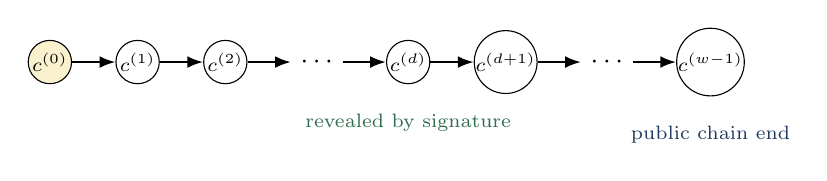
\begin{tikzpicture}[
  node distance=0.55cm,
  chain/.style={draw, circle, minimum size=0.55cm, inner sep=0pt, font=\scriptsize},
  arrow/.style={-{Latex[length=2mm]}, thick}
]
\node[chain, fill=qwpyellow!35] (c0) {\(c^{(0)}\)};
\node[chain, right=of c0] (c1) {\(c^{(1)}\)};
\node[chain, right=of c1] (c2) {\(c^{(2)}\)};
\node[right=of c2] (dots) {\(\cdots\)};
\node[chain, right=of dots] (cd) {\(c^{(d)}\)};
\node[chain, right=of cd] (cd1) {\(c^{(d+1)}\)};
\node[right=of cd1] (dots2) {\(\cdots\)};
\node[chain, right=of dots2] (cw) {\(c^{(w-1)}\)};
\draw[arrow] (c0) -- (c1);
\draw[arrow] (c1) -- (c2);
\draw[arrow] (c2) -- (dots);
\draw[arrow] (dots) -- (cd);
\draw[arrow] (cd) -- (cd1);
\draw[arrow] (cd1) -- (dots2);
\draw[arrow] (dots2) -- (cw);
\node[below=0.25cm of cd, font=\scriptsize, text=qwpgreen] {revealed by signature};
\node[below=0.25cm of cw, font=\scriptsize, text=qwpblue] {public chain end};
\end{tikzpicture}
\caption{A Winternitz chain. The signature reveals the value at the message
digit \(d\); verification recomputes \(w-1-d\) steps to the public end.}
\label{fig:wots}
\end{figure}

\begin{figure}[ht]
\centering
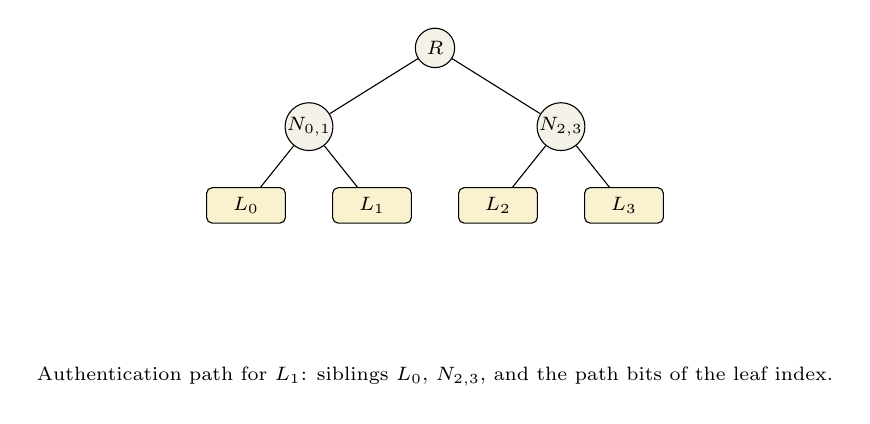
\begin{tikzpicture}[
  level distance=1.0cm,
  level 1/.style={sibling distance=3.2cm},
  level 2/.style={sibling distance=1.6cm},
  every node/.style={font=\scriptsize},
  leaf/.style={draw, rectangle, rounded corners=2pt, fill=qwpyellow!35, minimum width=1.0cm, minimum height=0.45cm},
  node/.style={draw, circle, fill=qwpgray, minimum size=0.5cm, inner sep=0pt},
  arrow/.style={-{Latex[length=1.8mm]}, thick}
]
\node[node] {\(R\)}
  child { node[node] {\(N_{0,1}\)}
    child { node[leaf] {\(L_0\)} }
    child { node[leaf] {\(L_1\)} }
  }
  child { node[node] {\(N_{2,3}\)}
    child { node[leaf] {\(L_2\)} }
    child { node[leaf] {\(L_3\)} }
  };
\node[below=1.7cm of current bounding box.south, font=\scriptsize, align=center]
  {Authentication path for \(L_1\): siblings \(L_0\), \(N_{2,3}\), and the path bits of the leaf index.};
\end{tikzpicture}
\caption{A Merkle authentication path. The verifier climbs from the leaf to the
root using the sibling at each level and the bits of the leaf index.}
\label{fig:merkle}
\end{figure}

\subsection{FORS and hypertrees}

A forest of few-time signatures (FORS) uses \(t\) trees of height \(h_{\mathrm{F}}\)
and \(2^{h_{\mathrm{F}}}\) leaves per tree. A message digest selects one leaf per
tree. The forest public key is
\[
\mathrm{FORS\_PK}
=
H_{\text{fors-pk}}(R_0\concat\cdots\concat R_{t-1}),
\]
where \(R_i\) is the Merkle root of tree \(i\). A hypertree of \(L\) layers and
subtree height \(h\) has total height \(H=Lh\). A path index
\(\mathrm{idx}\in\bits^H\) selects one leaf per layer. Layer \(\ell\) signs the
root of the tree below it; the top layer signs the public root.

\subsection{Concrete hash assumptions}

The proofs assume that BLAKE3 behaves as a PRF for the fixed derive-key
contexts, and that it is preimage- and collision-resistant at the stated output
length. For 256-bit outputs, the classical collision bound is about
\(2^{-128}\) by the birthday bound; for 512-bit outputs, about \(2^{-256}\).
These are assumptions, not theorems about BLAKE3. The implementation checks the
assumptions with known-answer tests and differential tests, not with a proof.

\part{Constructions}

\section{QHS-1}

\subsection{Parameters}

QHS-1 uses \(n=256\) bits, \(w=16\) (four-bit digits), \(67\) chains of length
\(15\), and a Merkle tree of height \(h=8\). The public and private keys are
\(64\) bytes; the signature is \(2{,}408\) bytes; the capacity is \(256\)
signatures per key.

\subsection{Key generation}

For a seed \(\mathrm{seed}\in\bits^{256}\) and leaf index \(i\in\{0,\dots,255\}\),
\[
s_{i,j}=H_{\text{secret}}(\mathrm{seed}\concat\langle i\rangle\concat\langle j\rangle),
\qquad j=0,\dots,66,
\]
\[
p_{i,j}=F^{15}(s_{i,j}),\qquad F(x)=H_{\text{chain}}(x),
\]
\[
P_i=H_{\text{wots}}(p_{i,0}\concat\cdots\concat p_{i,66}),
\]
\[
L_i=H_{\text{leaf}}(\langle i\rangle\concat P_i).
\]
The root is the Merkle root of \(L_0,\dots,L_{255}\). The private key stores the
seed and the counter; the public key stores the root and metadata.

\subsection{Message encoding}

For a message \(m\),
\[
D=H_{\text{message}}(m)\in\bits^{256}.
\]
Split \(D\) into \(64\) nibbles \(d_0,\dots,d_{63}\). The checksum is
\[
C=\sum_{k=0}^{63}(15-d_k)\in\{0,\dots,960\}.
\]
Encode \(C\) as three nibbles \(d_{64},d_{65},d_{66}\) in big-endian order. The
digit vector is \(d=(d_0,\dots,d_{66})\).

\subsection{Signing}

For the current counter \(i\), require \(i<256\). The signature is
\[
\sigma=(\mathrm{hdr},w_0,\dots,w_{66},\pi_i,\tau),
\]
where
\[
w_j=F^{d_j}(s_{i,j}),\qquad
\mathrm{hdr}=(\langle 1\rangle,\langle 1\rangle,\langle i\rangle),
\]
\(\pi_i\) is the eight-node authentication path, and \(\tau\) is the
four-byte format checksum
\[
\tau=H_{\text{checksum}}(\mathrm{hdr}\concat w_0\concat\cdots\concat w_{66}\concat\pi_i)_{[0,3]}.
\]
The counter is advanced and persisted before the signature is released.

\subsection{Verification}

Parse the header, leaf index, chain values, authentication path, and checksum.
Recompute \(d\). For each chain,
\[
p'_j=F^{15-d_j}(w_j),
\qquad
P'_i=H_{\text{wots}}(p'_0\concat\cdots\concat p'_{66}),
\]
\[
L'_i=H_{\text{leaf}}(\langle i\rangle\concat P'_i),
\qquad
R'=\mathrm{Climb}(L'_i,\pi_i,i).
\]
Accept iff \(R'=R\), the header is canonical, and the checksum matches.

\subsection{Size equation}

The signature size is
\[
4+67\cdot 32+8\cdot 32+4=2{,}408\text{ bytes}.
\]
The four-byte checksum is a corruption check, not an authenticator.

\section{QHS-2}

QHS-2 keeps the height-8 tree and capacity 256 but changes the digit base to
\(64\) and the chain parameters to \(45\) chains of length \(63\). The signature
is \(1{,}704\) bytes. The message encoding is
\[
D=H_{\text{message}}(m)\in\bits^{256},
\]
padded with two leading zero bits and split into \(43\) six-bit digits plus two
checksum digits. The checksum is
\[
C=\sum_{k=0}^{42}(63-d_k)\in\{0,\dots,2709\},
\]
encoded in two base-64 digits. The WOTS equations are
\[
s_{i,j}=H_{\text{secret}}(\mathrm{seed}\concat\langle i\rangle\concat\langle j\rangle),
\quad
p_{i,j}=F^{63}(s_{i,j}),
\quad
P_i=H_{\text{wots}}(p_{i,0}\concat\cdots\concat p_{i,44}).
\]
The signature size is
\[
4+45\cdot 32+8\cdot 32+4=1{,}704\text{ bytes}.
\]

\section{QHS-3 and QHS-3.1}

QHS-3 uses the QHS-2 WOTS parameters and a height-12 tree:
\[
N=2^{12}=4{,}096,\qquad
\text{signature}=4+45\cdot 32+12\cdot 32+4=1{,}832\text{ bytes}.
\]
The authentication path is \(384\) bytes. The capacity is \(4{,}096\)
signatures per key. The signing time is dominated by authentication-path
extraction; QHS-3.1 is the same signature with a \(262{,}180\)-byte public tree
cache, reducing signing to the WOTS work plus cache access.

Security is the same as QHS-2 except for the larger reduction loss
\[
4096\cdot 45\cdot 63\approx 2^{21.47},
\]
which is absorbed by the 256-bit hash output. The Merkle collision bound remains
about \(2^{-128}\) classically.

\section{QHS-4 and QHS-4.1}

\subsection{Parameters}

QHS-4 uses \(n=256\), \(45\) chains of length \(63\), a forest of \(16\) trees
of height \(8\), and a hypertree of \(8\) layers with subtree height \(8\),
for a total height \(64\). Keys are \(68\) bytes; signatures are \(18{,}216\)
bytes; there is no counter, cache, or state guard.

\subsection{Hypertree indexing}

A \(64\)-bit path \(\mathrm{idx}\) selects, for layer \(\ell=0,\dots,7\),
\[
i_\ell=(\mathrm{idx}\gg 8\ell)\mathbin{\&}255,
\qquad
t_\ell=\mathrm{idx}\gg 8(\ell+1)
\]
with \(t_7=0\). Layer \(0\) is the bottom layer; layer \(7\) contains the public
root.

\subsection{WOTS layer equations}

For layer \(\ell\), tree \(t\), leaf \(i\), chain \(j\):
\[
s_{\ell,t,i,j}
=
H_{\text{wots secret}}
(\mathrm{SK.seed}\concat\mathrm{PK.seed}\concat\langle\ell\rangle
\concat\langle t\rangle\concat\langle i\rangle\concat\langle j\rangle),
\]
\[
p_{\ell,t,i,j}=F^{63}(s_{\ell,t,i,j}),
\qquad
P_{\ell,t,i}=H_{\text{wots-pk}}(p_{\ell,t,i,0}\concat\cdots\concat p_{\ell,t,i,44}),
\]
\[
L_{\ell,t,i}=H_{\text{leaf}}(\langle\ell\rangle\concat\langle t\rangle
\concat\langle i\rangle\concat P_{\ell,t,i}).
\]
The layer message is the FORS public key at layer \(0\) and the child tree root
at higher layers. Upper-layer WOTS keys therefore sign a fixed value; reusing
them repeats the same deterministic signature.

\subsection{FORS equations}

For bottom tree \(t\) and leaf \(i\), FORS has 16 trees of 256 leaves:
\[
s_{a,b}=H_{\text{fors secret}}
(\mathrm{SK.seed}\concat\mathrm{PK.seed}\concat\langle t\rangle
\concat\langle i\rangle\concat\langle a\rangle\concat\langle b\rangle),
\]
\[
L_{a,b}=H_{\text{fors leaf}}(\langle a\rangle\concat\langle b\rangle\concat s_{a,b}),
\qquad
R_a=\mathrm{Merkle}_8(L_{a,0},\dots,L_{a,255}),
\]
\[
\mathrm{FORS\_PK}=H_{\text{fors-pk}}(R_0\concat\cdots\concat R_{15}).
\]
A FORS signature reveals one secret per tree plus its authentication path.

\subsection{Signature layout}

The signature is
\[
4\text{ header}+32\text{ randomizer}+4{,}608\text{ FORS}+13{,}568\text{ hypertree}+4\text{ checksum}
=18{,}216\text{ bytes}.
\]
The randomizer binds the message and the bottom path; the checksum covers the
first \(18{,}212\) bytes.

\subsection{QHS-4.1}

QHS-4.1 is the same construction with parallel subtree and forest generation.
The byte output is identical; the key and signature formats, proof, and security
bound are unchanged. The optimization is an engineering change, not a new
parameter set.

\section{QHS-4.2}

QHS-4.2 uses \(34\) chains of length \(255\), a forest of \(17\) trees of height
\(8\), and a hypertree of \(7\) layers of height \(8\), total height \(56\).
The signature is
\[
4+32+17\cdot(32+8\cdot 32)+7\cdot(34\cdot 32+8\cdot 32)+4
=14{,}344\text{ bytes}.
\]
The indexing equations are the same as QHS-4 with
\(\mathrm{idx}\in\bits^{56}\), \(i_\ell=(\mathrm{idx}\gg 8\ell)\&255\),
\(t_\ell=\mathrm{idx}\gg 8(\ell+1)\), and \(\ell=0,\dots,6\). The FORS digest
selects \(17\) indices rather than \(16\). The security analysis uses the same
lemmas with \(56\)-bit paths and \(17\)-tree forests.

\section{QHS-5}

\subsection{512-bit hash mode}

QHS-5 uses the 512-bit mode
\[
H64_d(x)=H_{d,0}(0x00\concat x)\concat H_{d,1}(0x01\concat x).
\]
The two halves are independent BLAKE3 instances with distinct domain tags. The
output gives 512-bit preimage resistance and 256-bit collision resistance in the
classical model, and approximately 256-bit preimage and 128-bit collision
resistance in the quantum model.

\subsection{Parameters and equations}

QHS-5 uses \(89\) chains of length \(63\): \(86\) message digits plus \(3\)
checksum digits. Keys are \(72\) bytes; signatures are \(6{,}216\) bytes; the
capacity is \(256\) signatures per key. For leaf \(i\) and chain \(j\):
\[
s_{i,j}=H64_{\text{secret}}(\mathrm{seed}\concat\langle i\rangle\concat\langle j\rangle),
\quad
p_{i,j}=F^{63}(s_{i,j}),
\]
\[
P_i=H64_{\text{wots-pk}}(p_{i,0}\concat\cdots\concat p_{i,88}),
\quad
L_i=H64_{\text{leaf}}(\langle i\rangle\concat P_i).
\]
The public key is the height-8 Merkle root.

\subsection{Message digits and checksum}

The digest is
\[
D=H64_{\text{message}}(m)\in\bits^{512}.
\]
The first \(86\) base-64 digits encode the full digest with four leading zero
bits. The checksum is
\[
C=\sum_{k=0}^{85}(63-d_k)\in\{0,\dots,5418\},
\]
encoded in three base-64 digits:
\[
d_{86}=C\gg 12,\qquad
d_{87}=(C\gg 6)\&63,\qquad
d_{88}=C\&63.
\]
The \(89\)-digit vector is the WOTS message.

\subsection{Signature layout}

The signature is
\[
4+89\cdot 64+8\cdot 64+4=6{,}216\text{ bytes}.
\]
The checksum covers the first \(6{,}212\) bytes.

\section{QHS-6}

QHS-6 composes QHS-5 with Ed25519. The public key is \(108\) bytes, the private
key is \(108\) bytes, and the signature is \(6{,}284\) bytes. The layout is
\[
4\text{ header}+72\text{ QHS-5 public}+32\text{ Ed25519 public}
\]
for the public key, and
\[
4\text{ header}+72\text{ QHS-5 private}+32\text{ Ed25519 seed}
\]
for the private key. The signature layout is
\[
4\text{ header}+6{,}216\text{ QHS-5 signature}+64\text{ Ed25519 signature}.
\]

\subsection{Transcript binding}

For message \(m\), QHS-5 public key \(P_5\), and Ed25519 public key \(P_E\),
\[
T=H64_{\text{transcript}}(P_5\concat P_E\concat m).
\]
Both components sign \(T\). The transcript prevents component mixing across
messages, keys, and versions. QHS-5 signs the transcript with its next leaf;
Ed25519 signs it deterministically.

\subsection{Verification predicate}

Parse the hybrid key and signature. Check the header, leaf index, and exact
lengths. Require the hybrid leaf index to equal the QHS-5 component leaf index.
Recompute
\[
T=H64_{\text{transcript}}(P_5\concat P_E\concat m).
\]
Accept iff
\[
\Ver_{\mathrm{QHS5}}(P_5,T,\sigma_5)=\acc
\quad\wedge\quad
\Ver_{\mathrm{Ed25519}}(P_E,T,\sigma_E)=\acc.
\]

\section{QHS-E}

QHS-E is the verifier-only profile of QHS-1, QHS-2, QHS-3, and QHS-3.1. It
accepts the same public keys and signatures and uses the same equations and
domain contexts. Its security statement is the differential equivalence
\[
\forall (pk,m,\sigma):\quad
\Ver_{E,v}(pk,m,\sigma)=\Ver_{v}(pk,m,\sigma),
\]
for each base version \(v\). The profile has no key generation, signing, cache,
or state guard. It is no-standard-library, allocation-free, and forbids unsafe
code. The measured code size is \(12{,}771\) bytes on thumbv7em and \(14{,}247\)
bytes on riscv32imac; the peak verifier frame is about six kilobytes, driven by
the BLAKE3 hasher.

\section{Parameter synthesis and optimization}

\subsection{Size equations}

The stateful signature sizes are
\[
4+\ell\cdot 32+h\cdot 32+4
\]
for 32-byte chains, and
\[
4+\ell\cdot 64+h\cdot 64+4
\]
for 64-byte chains, where \(\ell\) is the number of chains and \(h\) the tree
height. The stateless sizes add the forest and layer terms:
\[
4+32+t(32+32h_{\mathrm F})+L(\ell\cdot 32+32h)+4
\]
for QHS-4-style signatures, and analogously for QHS-4.2. These equations were
used to choose the parameter sets in Table~\ref{tab:params}.

\subsection{Latency model}

The signing cost is dominated by chain evaluations and tree generation. For a
stateful version with \(\ell\) chains and \(w\) steps, the worst-case chain work
is at most \(\ell w\) evaluations. For a stateless version, the dominant term is
the generation of the forest and hypertree subtrees; parallelization reduces
the wall-clock time without changing the byte output. The measured numbers are
reported in Part VI.

\subsection{Capacity}

The stateful capacity is \(2^h\) with a two-byte counter for \(h\le 15\). QHS-1
and QHS-2 use \(h=8\); QHS-3 and QHS-3.1 use \(h=12\); QHS-5 uses \(h=8\). The
stateless capacity is bounded by the path-collision and FORS-reuse bounds; the
documented target is about one million signatures per key for QHS-4 and
QHS-4.2.

\begin{table}[ht]
\centering
\caption{Parameter summary. The table is the compact form of the equations in
this part.}
\label{tab:params}
\small
\begin{tabularx}{\textwidth}{@{}l l r r r r@{}}
\toprule
Version & Type & Chains & Chain length & Tree/height & Signature\\
\midrule
QHS-1 & stateful & 67 & 15 & 8 & 2,408 B\\
QHS-2 & stateful & 45 & 63 & 8 & 1,704 B\\
QHS-3 & stateful & 45 & 63 & 12 & 1,832 B\\
QHS-3.1 & stateful & 45 & 63 & 12 & 1,832 B\\
QHS-4 & stateless & 45 & 63 & 8 layers, 64 total & 18,216 B\\
QHS-4.1 & stateless & 45 & 63 & 8 layers, 64 total & 18,216 B\\
QHS-4.2 & stateless & 34 & 255 & 7 layers, 56 total & 14,344 B\\
QHS-5 & stateful & 89 & 63 & 8 & 6,216 B\\
QHS-6 & hybrid & 89 & 63 & 8 & 6,284 B\\
QHS-E & verifier & base & base & base & base\\
\bottomrule
\end{tabularx}
\end{table}

\part{Security analysis}

\section{Security definitions and reduction structure}

The reductions follow a common pattern. A forgery is classified as a used-leaf
forgery, an unused-leaf forgery, a path forgery, a forest forgery, a transcript
collision, or a parser/checksum failure. Each cryptographic class is mapped to a
preimage, second-preimage, or collision event for the underlying hash. The
reduction guesses the relevant chain, leaf, tree, or path; the guessing loss is
absorbed by the hash margin.

\subsection{Reduction diagram}

\begin{figure}[ht]
\centering
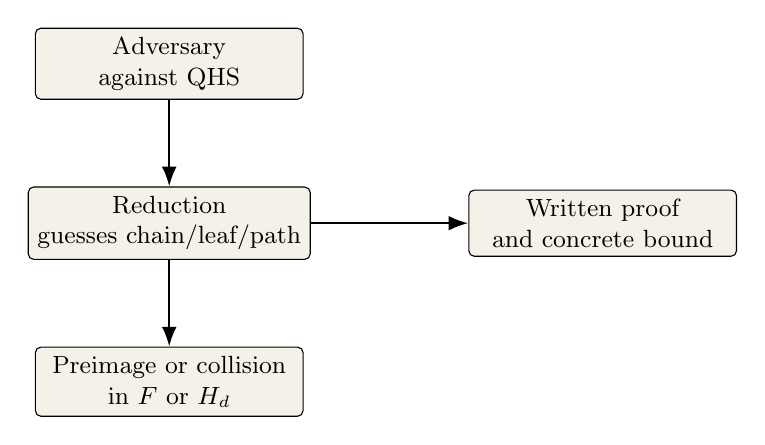
\begin{tikzpicture}[
  node distance=1.1cm and 2.0cm,
  box/.style={draw, rounded corners=2pt, align=center, minimum width=3.4cm, minimum height=0.8cm, font=\small},
  arrow/.style={-{Latex[length=2.5mm]}, thick}
]
\node[box, fill=qwpgray] (adv) {Adversary\\against QHS};
\node[box, fill=qwpgray, below=of adv] (red) {Reduction\\guesses chain/leaf/path};
\node[box, fill=qwpgray, below=of red] (hash) {Preimage or collision\\in \(F\) or \(H_d\)};
\node[box, fill=qwpgray, right=of red] (proof) {Written proof\\and concrete bound};
\draw[arrow] (adv) -- (red);
\draw[arrow] (red) -- (hash);
\draw[arrow] (red) -- (proof);
\end{tikzpicture}
\caption{The common reduction shape. The reduction guesses the object that the
forgery must reuse, embeds a challenge, and turns the forgery into a preimage or
collision.}
\label{fig:reduction}
\end{figure}

\section{Stateful bounds}

\subsection{QHS-1}

The QHS-1 proof classifies a forgery into a used-leaf forgery, an unused-leaf
forgery, or a path forgery. The used-leaf reduction guesses one of \(67\cdot15\)
chain positions and embeds a challenge. The reduction loss is
\[
L_1=256\cdot67\cdot15\approx 2^{18}.
\]
The concrete bound is stated as
\[
\Adv^{\EUF}_{\mathrm{QHS-1}}(\mathcal{A})
\le
L_1\left(\Adv^{\pre}_{F}(\mathcal{B}_1)
+\Adv^{\coll}_{H}(\mathcal{B}_2)\right),
\]
with the factor absorbed by the 256-bit hash output. The WOTS preimage margin is
approximately
\[
256-18=238\text{ bits},
\]
and the Merkle collision bound is approximately \(2^{-128}\) classically.

\subsection{QHS-2}

For QHS-2 the reduction loss is
\[
L_2=256\cdot45\cdot63\approx 2^{19.47},
\]
so the WOTS preimage margin is approximately
\[
256-19.47\approx 236.5\text{ bits}.
\]
The Merkle collision bound is again about \(2^{-128}\) classically.

\subsection{QHS-3 and QHS-3.1}

For QHS-3 the capacity is \(4{,}096\), so the reduction loss is
\[
L_3=4096\cdot45\cdot63\approx 2^{21.47}.
\]
The WOTS preimage margin is approximately
\[
256-21.47\approx 234.5\text{ bits}.
\]
QHS-3.1 uses the same signature and proof; only the authentication-path
extraction changes.

\subsection{Stateful invariant}

The bounds assume the leaf invariant. A leaf reuse invalidates the one-time
argument. The implementation enforces a monotone counter, an atomic key update,
a lock file, and a keyed state guard. The state guard detects a guard counter
ahead of the key counter and refuses a corrupt or missing guard for an advanced
key. It cannot detect a rollback of both the key and the guard; that requires
external trusted state.

\section{Stateless bounds}

\subsection{QHS-4}

For a single FORS key, after \(\gamma\) signatures on the same bottom leaf, the
adversary has seen at most \(\gamma\) leaves per FORS tree. A forgery requires
the message digest to select only revealed leaves in all \(16\) trees:
\[
\Prb[\text{FORS forgery}\mid \text{fixed leaf}]
\le
\left(\frac{\gamma}{256}\right)^{16}.
\]
For \(\gamma=1\) this is \(2^{-128}\); for \(\gamma=2\) it is \(2^{-112}\).

To use a revealed FORS key, the forgery must first hit one of the \(q\) used
bottom leaves. The bottom path is a \(64\)-bit value, so
\[
\Prb[\text{hit used leaf}]
\le
\frac{q}{2^{64}}.
\]
For \(q\le 2^{20}\) and \(\gamma=1\),
\[
\Prb[\text{FORS forgery}]
\le
\frac{q}{2^{64}}\cdot 2^{-128}
=
2^{-172}.
\]

\subsection{Path reuse}

Two signatures share the full \(64\)-bit path with probability at most
\[
\Prb[\text{path collision}]
\le
\frac{q(q-1)}{2^{65}}.
\]
For \(q\le 2^{20}\), this is at most \(2^{-25}\). If a collision occurs, the
FORS key is used twice, and the second-signature forgery probability is at most
\(2^{-112}\). The product is
\[
2^{-25}\cdot 2^{-112}=2^{-137}.
\]
Upper-layer WOTS keys sign fixed roots, so their reuse is harmless.

\subsection{Merkle collision}

A forged authentication path that reaches the same root from a different leaf
yields a collision in \(H_{\text{leaf}}\) or \(H_{\text{node}}\). With a 256-bit
output, the classical collision bound is about \(2^{-128}\). The dominant
classical term is therefore the 128-bit collision bound; QHS-4 targets
128-bit classical security for \(q\le 2^{20}\).

\subsection{QHS-4.2}

QHS-4.2 uses a \(56\)-bit path and \(17\) FORS trees:
\[
\Prb[\text{FORS forgery}\mid \text{fixed leaf}]
\le
\left(\frac{\gamma}{256}\right)^{17},
\]
so for \(\gamma=1\) the fixed-leaf bound is \(2^{-136}\). The used-leaf hit
probability is at most \(q/2^{56}\), and for \(q\le 2^{20}\)
\[
\frac{q}{2^{56}}\cdot 2^{-136}=2^{-172}.
\]
The path-collision bound is
\[
\frac{q(q-1)}{2^{57}}\le 2^{-17}
\]
for \(q\le 2^{20}\), and the reuse product is
\[
2^{-17}\cdot 2^{-119}=2^{-136}.
\]
The Merkle collision bound is again about \(2^{-128}\) classically.

\subsection{Theorem statements}

\begin{theorem}[QHS-1 EUF-CMA]
For at most \(256\) signing queries with distinct leaves, QHS-1 is
existentially unforgeable under chosen-message attack assuming BLAKE3 is
preimage- and collision-resistant for the fixed contexts and the stateful leaf
invariant holds. In the reduction,
\[
\Adv^{\EUF}_{\mathrm{QHS-1}}(\mathcal{A})
\le
2^{18}\left(\Adv^{\pre}_{F}(\mathcal{B}_1)
+\Adv^{\coll}_{H}(\mathcal{B}_2)\right).
\]
\end{theorem}
\begin{proof}[Proof sketch]
Classify a forgery as a used-leaf, unused-leaf, or path forgery. The used-leaf
case guesses one of the \(67\cdot15\) chain positions and embeds a challenge;
the unused-leaf case is at least as hard without a signing query; the path case
yields a collision in the leaf or node hash. The guessing loss is
\(256\cdot67\cdot15\approx2^{18}\), absorbed by the 256-bit output.
\end{proof}

\begin{theorem}[QHS-2 EUF-CMA]
For at most \(256\) signing queries with distinct leaves, QHS-2 is EUF-CMA
under the same assumptions, with reduction loss
\[
2^{19.47}=256\cdot45\cdot63.
\]
\end{theorem}
\begin{proof}[Proof sketch]
The proof is the QHS-1 argument with 45 chains of length 63 and the base-64
digit/checksum encoding. The used-leaf guess is over \(45\cdot63\) positions.
\end{proof}

\begin{theorem}[QHS-3 and QHS-3.1 EUF-CMA]
For at most \(4{,}096\) signing queries with distinct leaves, QHS-3 and
QHS-3.1 are EUF-CMA under the same assumptions, with reduction loss
\[
2^{21.47}=4096\cdot45\cdot63.
\]
\end{theorem}
\begin{proof}[Proof sketch]
The proof is the QHS-2 argument over a height-12 tree. QHS-3.1 uses the same
signature, format, and proof; the tree cache changes only authentication-path
extraction.
\end{proof}

\begin{theorem}[QHS-4 and QHS-4.1 EUF-CMA]
For at most \(q\le2^{20}\) signing queries, QHS-4 and QHS-4.1 are EUF-CMA
assuming BLAKE3 is a PRF and is preimage- and collision-resistant. The
dominant terms are
\[
\frac{q}{2^{64}}\cdot2^{-128}=2^{-172},
\qquad
\frac{q(q-1)}{2^{65}}\le2^{-25},
\qquad
2^{-25}\cdot2^{-112}=2^{-137},
\]
and the classical Merkle/FORS collision term about \(2^{-128}\).
\end{theorem}
\begin{proof}[Proof sketch]
A forgery is a FORS forgery, a fixed-message WOTS forgery, a path forgery, or a
checksum/parser failure. FORS reuse requires hitting a used 64-bit bottom path
and then selecting revealed leaves in all 16 trees. Upper-layer WOTS keys sign
fixed roots, so their reuse is harmless. The collision cap is the 128-bit
Merkle/FORS term.
\end{proof}

\begin{theorem}[QHS-4.2 EUF-CMA]
For at most \(q\le2^{20}\) signing queries, QHS-4.2 is EUF-CMA with
\[
\frac{q}{2^{56}}\cdot2^{-136}=2^{-172},
\qquad
\frac{q(q-1)}{2^{57}}\le2^{-17},
\qquad
2^{-17}\cdot2^{-119}=2^{-136},
\]
and the same 128-bit collision cap.
\end{theorem}
\begin{proof}[Proof sketch]
The proof is the QHS-4 argument with a 56-bit path and 17 FORS trees. The
smaller path increases the collision probability but the FORS reuse term and
the 128-bit collision cap still dominate the classical bound.
\end{proof}

\begin{theorem}[QHS-5 EUF-CMA]
For at most 256 signing queries with distinct leaves, QHS-5 is EUF-CMA with a
512-bit digest. The WOTS fixed-message advantage is about
\[
2^{-512+12.45}=2^{-499.55},
\]
capped by the 256-bit classical collision term and the approximately 128-bit
quantum collision term.
\end{theorem}
\begin{proof}[Proof sketch]
The digit encoding is injective over the 512-bit digest. A used-leaf forgery
requires a chain preimage or a digit collision; an unused-leaf forgery is at
least as hard; a path forgery yields a Merkle collision. The stateful leaf
invariant is assumed.
\end{proof}

\begin{theorem}[QHS-6 hybrid unforgeability]
QHS-6 is EUF-CMA if either QHS-5 or Ed25519 is EUF-CMA and the transcript hash
is collision-resistant. In particular,
\[
\Adv^{\EUF}_{\mathrm{hyb}}(\mathcal{A})
\le
\Adv^{\EUF}_{\mathrm{QHS5}}(\mathcal{B}_1)
+\Adv^{\coll}_{H64}(\mathcal{B}_2),
\]
and symmetrically for Ed25519.
\end{theorem}
\begin{proof}[Proof sketch]
A hybrid forgery contains both component signatures on the same transcript
\(T^*\). If the signer never signed \(T^*\), one component is a forgery. If it
signed a different transcript, the acceptance implies a transcript collision.
The transcript binds both public keys and the message, preventing component
mixing.
\end{proof}

\begin{theorem}[QHS-E differential equivalence]
For every fixed-format public key, message, and signature,
\[
\Ver_{E,v}(pk,m,\sigma)=\Ver_{v}(pk,m,\sigma)
\]
for each base version \(v\in\{\mathrm{QHS-1},\mathrm{QHS-2},\mathrm{QHS-3},\mathrm{QHS-3.1}\}\).
\end{theorem}
\begin{proof}[Proof sketch]
Both verifiers check the same headers, leaf bounds, checksum range, digit
encoding, chain counts and lengths, leaf and node contexts, and Merkle path
bits. The differential tests, full bit sweep, structural transplant suite, and
public-key mutation suite are the implementation evidence.
\end{proof}

\section{512-bit margin}

QHS-5 uses a 512-bit output. The digit encoding is injective over the 512-bit
digest, so a digit collision implies a hash collision. The WOTS reduction loss
is
\[
89\cdot 63=5{,}607\approx 2^{12.45}.
\]
The fixed-message WOTS advantage is approximately
\[
2^{-512+12.45}=2^{-499.55},
\]
and the classical collision bound is about \(2^{-256}\). The overall classical
target is 256 bits; the quantum collision bound is about \(2^{-128}\), which is
the limiting quantum term. The message-digit, WOTS, and Merkle terms therefore
support the stated 256-bit classical and approximately 128-bit quantum claim.

\section{Hybrid composition}

For QHS-6, the transcript is
\[
T=H64_{\text{transcript}}(P_5\concat P_E\concat m).
\]
A hybrid forgery accepted by the verifier contains a valid QHS-5 signature on
\(T^*\) and a valid Ed25519 signature on \(T^*\). If the signer never signed
\(T^*\), the QHS-5 part is a QHS-5 forgery and the Ed25519 part is an Ed25519
forgery. If the signer signed a different transcript that collides with
\(T^*\), the forgery implies a transcript collision. Therefore
\[
\Adv^{\EUF}_{\mathrm{hyb}}(\mathcal{A})
\le
\Adv^{\EUF}_{\mathrm{QHS5}}(\mathcal{B}_1)
+
\Adv^{\coll}_{H64}(\mathcal{B}_2),
\]
and symmetrically
\[
\Adv^{\EUF}_{\mathrm{hyb}}(\mathcal{A})
\le
\Adv^{\EUF}_{\mathrm{Ed25519}}(\mathcal{B}_3)
+
\Adv^{\coll}_{H64}(\mathcal{B}_2).
\]
The hybrid is secure if either component is secure. A quantum break of Ed25519
does not help forge the QHS-5 component, so the hybrid retains the QHS-5 quantum
margin.

\section{Differential equivalence of QHS-E}

QHS-E is a verifier-only implementation. The equivalence statement is
\[
\forall (pk,m,\sigma):\quad
\Ver_{E,v}(pk,m,\sigma)=\Ver_{v}(pk,m,\sigma).
\]
The proof is by case analysis on the fixed layout: both implementations check
the same header, leaf bound, checksum range, digit encoding, chain length, chain
count, leaf and node contexts, and Merkle path bits. The evidence is the
differential test suite, the full bit sweep, the structural transplant suite,
and the public-key mutation suite. A divergence would be an implementation bug,
not a new assumption.

\section{Concrete security summary}

\begin{table}[ht]
\centering
\caption{Concrete security claims and dominant terms. These are design claims
supported by the written proofs and local evidence, not an external
certification.}
\label{tab:securitybounds}
\small
\begin{tabularx}{\textwidth}{@{}l l l X@{}}
\toprule
Version & Classical & Quantum & Dominant bound\\
\midrule
QHS-1 & at least 128-bit & at least 64-bit & 128-bit Merkle collision; WOTS preimage margin about 238 bits.\\
QHS-2 & at least 128-bit & at least 64-bit & 128-bit Merkle collision; WOTS preimage margin about 236.5 bits.\\
QHS-3/3.1 & at least 128-bit & at least 64-bit & 128-bit Merkle collision; WOTS preimage margin about 234.5 bits.\\
QHS-4 & 128-bit for \(q\le 2^{20}\) & at least 64-bit & 128-bit Merkle/FORS collision; FORS reuse \(2^{-172}\); path reuse \(2^{-137}\).\\
QHS-4.2 & 128-bit for \(q\le 2^{20}\) & at least 64-bit & 128-bit collision; FORS reuse \(2^{-172}\); path reuse \(2^{-136}\).\\
QHS-5 & 256-bit & about 128-bit & 256-bit collision; WOTS preimage about \(2^{-499.5}\).\\
QHS-6 & QHS-5 or Ed25519 & QHS-5 or Ed25519 & Hybrid composition plus transcript collision.\\
QHS-E & same as base & same as base & Differential equivalence; no new assumption.\\
\bottomrule
\end{tabularx}
\end{table}

\part{Implementation and code standard}

\section{Engineering model}

\subsection{State machine}

The stateful signer is a state machine with states \emph{ready},
\emph{signing}, \emph{persisted}, and \emph{exhausted}. A signing request is
accepted only in \emph{ready}. The counter is advanced, the key is written
atomically, the state guard is written, and only then is the signature released.
A crash before the signature write consumes a leaf but does not reuse one. A
crash after the key write but before the guard write leaves the guard behind;
the next signing request catches the guard up. A guard ahead of the key is
refused as a rollback signal.

\begin{figure}[ht]
\centering
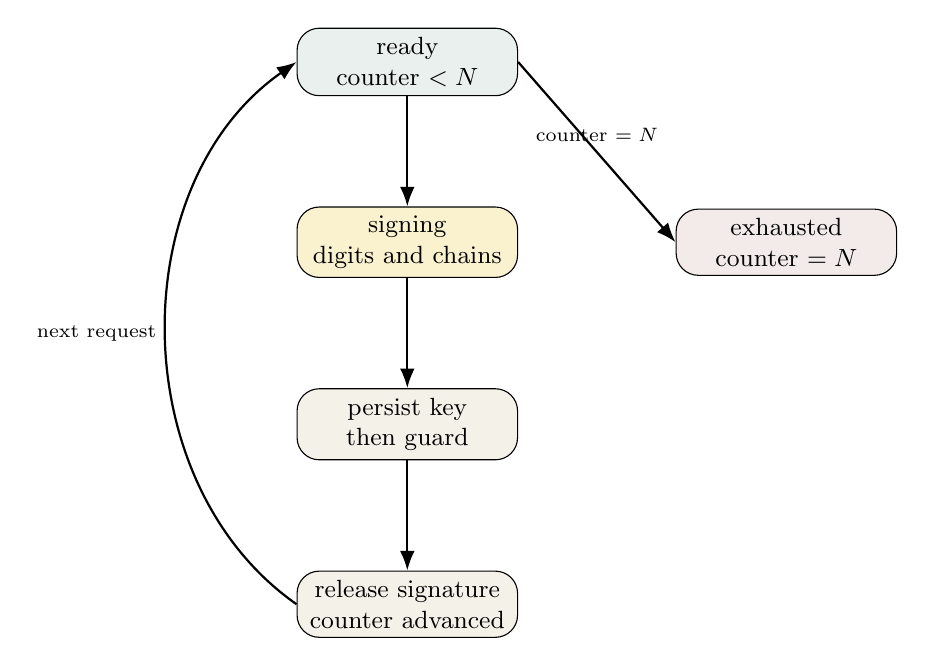
\begin{tikzpicture}[
  node distance=1.4cm and 2.0cm,
  state/.style={draw, rounded corners=8pt, minimum width=2.8cm, minimum height=0.8cm, align=center, font=\small},
  arrow/.style={-{Latex[length=2.5mm]}, thick}
]
\node[state, fill=qwpgreen!10] (ready) {ready\\counter \(<N\)};
\node[state, fill=qwpyellow!35, below=of ready] (signing) {signing\\digits and chains};
\node[state, fill=qwpgray, below=of signing] (persist) {persist key\\then guard};
\node[state, fill=qwpgray, below=of persist] (release) {release signature\\counter advanced};
\node[state, fill=qwpred!10, right=of signing] (exhausted) {exhausted\\counter \(=N\)};
\draw[arrow] (ready) -- (signing);
\draw[arrow] (signing) -- (persist);
\draw[arrow] (persist) -- (release);
\draw[arrow] (release.west) to[bend left=55] node[left,font=\scriptsize]{next request} (ready.west);
\draw[arrow] (ready.east) -- node[above,font=\scriptsize]{counter \(=N\)} (exhausted.west);
\end{tikzpicture}
\caption{Stateful signing order. The key is persisted before the signature is
released; a crash consumes a leaf rather than reusing it.}
\label{fig:state}
\end{figure}

\subsection{Atomic persistence}

The key update uses a temporary file, a synchronous flush, an atomic rename, and
private permissions. A lock file serializes cooperating signers. The state guard
is a keyed record containing the key header and the counter. A guard ahead of the
key counter is a rollback signal; a corrupt guard is a hard error; a missing
guard is a hard error for an advanced key. A missing guard at counter zero is
treated as a fresh key.

\subsection{Cache authentication}

The public-leaf and tree caches are versioned, fingerprinted with a
derive-key value of the seed, and authenticated with a keyed message
authentication code. The caches contain public Merkle data only. A corrupt or
foreign cache is rejected and recomputed. A cache from another key fails the
fingerprint or the MAC.

\subsection{Constant-time posture}

The field, scalar, and Edwards arithmetic avoid secret-dependent branches. The
verifier operates on public data. Timing is measured with a Welch harness and
with dudect. The QHS-E valid-path probes show no statistically significant
separation on the reference host; the positive control shows that the harness
detects early-rejection differences. Verification is public-data work, so the
early-rejection difference is not treated as a secret leak.

\section{The code standard}

\subsection{Policy levels}

The code standard is a compiler-enforced policy. Every production crate denies
the broad Clippy families \emph{all}, \emph{pedantic}, \emph{nursery}, and
\emph{cargo}. The production crypto core additionally denies allocation and
standard-library leakage, raw indexing, unwrap/expect/panic/todo/unimplemented/
unreachable, unchecked casts and lossy casts, floating-point arithmetic, missing
inline annotations on public items, and non-exhaustive structs and enums. The
additional hardening set covers arithmetic side effects where applicable,
panic-in-result, unwrap-in-result, allow attributes without reasons, debug
macros, process exit, memory forget, direct printing, missing documentation,
missing debug implementations, rustdoc, unreachable public items, unused
results, ignored must-use values, non-ASCII identifiers, and obsolete edition
and lifetime idioms.

\begin{table}[ht]
\centering
\caption{Code-standard levels and their intent.}
\label{tab:lintlevels}
\small
\begin{tabularx}{\textwidth}{@{}p{1.0cm}p{3.0cm}Y@{}}
\toprule
Level & Focus & Controls and intent\\
\midrule
1 & Default lax patterns & all, pedantic, nursery, cargo: broad complexity, conversion, documentation, and packaging hygiene.\\
2 & Core isolation & allocation and std isolation: keep the crypto core free of hidden runtime layers.\\
3 & Panic matrix & unwrap, expect, indexing, panic, todo, unimplemented, unreachable: remove compiled crash branches and unchecked array access.\\
4 & Casts and side channels & as conversions, lossless/truncating/wrapping casts, floating point: force explicit bounded conversions and deterministic integer math.\\
5 & Compiler shape & missing inline on public items, exhaustive structs and enums: make public boundaries and type shape explicit.\\
6 & Additional hardening & arithmetic side effects where applicable, panic/unwrap in result, allow reasons, debug macros, exit, forget, printing, docs/debug, rustdoc, visibility, unused results, lifetimes.\\
\bottomrule
\end{tabularx}
\end{table}

\subsection{Crate classification}

\begin{table}[ht]
\centering
\caption{Crate classes and code-standard posture.}
\label{tab:crates}
\small
\begin{tabularx}{\textwidth}{@{}l l c c Y@{}}
\toprule
Crate & Class & No-std & Unsafe forbidden & Posture\\
\midrule
qwp-core & production core & Yes & Yes & Full strict set; cargo metadata allow.\\
qwp-hash & production core & Yes & Yes & Full strict set; cargo metadata allow.\\
qwp-classical & production core & Yes & Yes & Full strict set; style-only allows and documented arithmetic exception.\\
qwp-crypto & production core & Yes & Yes & Full strict set; cargo metadata allow.\\
qwp-e & verifier profile & Yes & Yes & Full strict set; cargo metadata allow.\\
qwp-platform & host adapter & No & Yes & Std use intentional; security lints.\\
qwp-cli & host CLI & No & Yes & Std and printing allows with reasons.\\
qwp-attacks & attack harness & No & Yes & Std and printing allows with reasons.\\
qwp-bench & benchmark & No & Yes & Reduced set for timing.\\
qwp-tests & test/fuzz harness & No & Yes & Reduced set for the harness.\\
qwp-verify & Kani harness & Yes & Yes & Proof profile.\\
qwp-e-size & evidence staticlib & Yes & Yes & Size profile.\\
\bottomrule
\end{tabularx}
\end{table}

\subsection{Compliance and exceptions}

The production crates are clean under the strict set. The classical crate keeps
style-only exceptions for conventional single-letter names in SHA-512 and
Edwards formulas, grouped field literals, explicit internal visibility, and
cargo metadata. It has no indexing, cast, or unchecked-arithmetic exception. The
host tools use reduced sets because they are not production cryptographic code.
The proof and size crates are evidence profiles, not shipping libraries.

\subsection{Runnable policy}

The repository contains a code-standard script that runs formatting, Clippy with
warnings denied, the release test suite, dependency isolation, an unsafe-code
scan, and Kani. The full mode adds code size, timing, and coverage. The audit
document records the evidence and the remaining exceptions. The policy is
therefore a command and a table, not a statement of intent.

\section{Error model and panic freedom}

Public APIs return typed errors. Fixed-layout parsers check exact lengths and
headers. Production code avoids unwrap, expect, raw indexing, and panic. The
attack harness deliberately feeds malformed bytes and requires an error rather
than a panic. The fuzz driver catches panics per iteration and exits non-zero if
one occurs. The code standard denies the panic-producing constructs at compile
time; the tests and fuzzer check the remaining runtime paths.

\part{Verification methodology}

\section{Assurance model}

No single tool proves a cryptographic implementation. The project uses layers:
functional tests, differential tests, property tests, fuzzers, model checkers,
deductive tools, temporal analysis, concurrency modeling, timing analysis,
assembly inspection, undefined-behavior checking, coverage, mutation testing,
size and stack measurement, and soaks. Each layer has a stated scope.

\begin{figure}[ht]
\centering
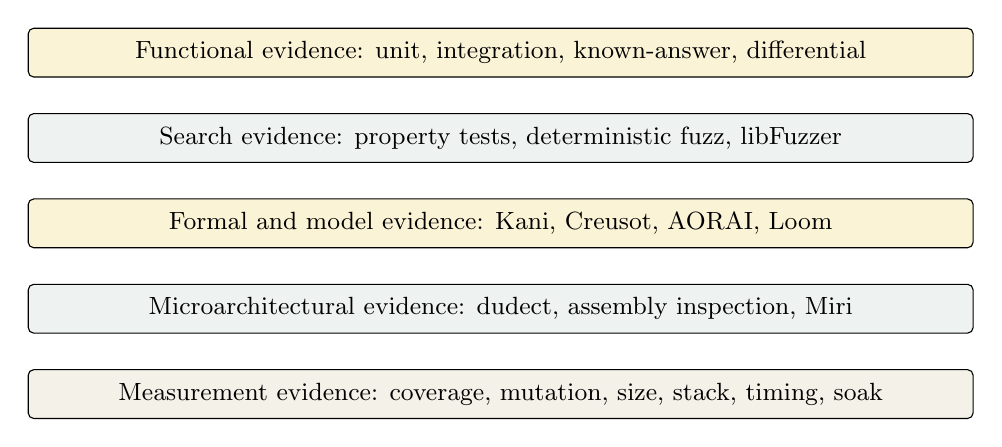
\begin{tikzpicture}[
  node distance=0.45cm,
  layer/.style={draw, rounded corners=2pt, minimum width=12.0cm, minimum height=0.62cm, align=center, font=\small},
  l1/.style={layer, fill=qwpyellow!30},
  l2/.style={layer, fill=qwpgreen!8},
  l3/.style={layer, fill=qwpgray}
]
\node[l1] (a) {Functional evidence: unit, integration, known-answer, differential};
\node[l2, below=of a] (b) {Search evidence: property tests, deterministic fuzz, libFuzzer};
\node[l1, below=of b] (c) {Formal and model evidence: Kani, Creusot, AORAI, Loom};
\node[l2, below=of c] (d) {Microarchitectural evidence: dudect, assembly inspection, Miri};
\node[l3, below=of d] (e) {Measurement evidence: coverage, mutation, size, stack, timing, soak};
\end{tikzpicture}
\caption{The layered assurance model. Each layer answers a different question;
none replaces an independent audit.}
\label{fig:assurance}
\end{figure}

\section{Functional evidence}

The release suite contains 308 tests. It covers key generation, signing,
verification, parsing, serialization, caches, state guards, command-line
behavior, known-answer vectors, RFC 8032 Ed25519 vectors, and negative cases.
The tests run in debug and release profiles. The release profile is used for
the evidence snapshot.

Differential testing compares QHS-E with the base verifiers for valid
signatures, tampered signatures, wrong messages, wrong keys, cross-version
inputs, random signatures, multiple leaves, and non-canonical public-key tails.
The differential suite is the main evidence for the equivalence lemma.

\section{Property-based and fuzz evidence}

The proptest suite contains five properties with 64 cases each, plus four
regression tests. It checks valid/invalid message behavior, single-byte mutation
rejection, parser round-trips, and QHS-6 hybrid behavior.

The deterministic fuzz driver exercises all versions in one process. It generates
random keys, messages, signatures, caches, and state files; it checks round-trip
behavior, parser behavior, and panic freedom. It accepts a seed and prints
progress every sixty seconds. The libFuzzer targets cover the QHS-E verifier,
the fixed and variable signature parsers, and the QHS-6 hybrid parser. The latest
QHS-E run completed 17,961,180 executions in 61 seconds with no crash; the parser
targets completed about 29 million executions each in 46 seconds.

\section{Formal and model evidence}

Kani proves 24 parser and bounds harnesses across QHS-1, QHS-2, QHS-3, QHS-3.1,
QHS-4, QHS-4.2, QHS-5, and QHS-6. The harnesses cover fixed-layout parsing,
length checks, header checks, and index bounds. Kani does not prove the full
functional correctness of BLAKE3 or the complete verifier.

Creusot proves seven contracts on a model of the QHS-E digit, checksum, and
Merkle arithmetic: base-64 digits below 64, hexadecimal digits below 16,
checksum sums within bounds, authentication-path offsets below 384, and the leaf
index predicates for 256 and 4,096. AORAI checks a C model of the verification
order; the run proves 1,050 of 1,051 goals, with one tool-generated typing
timeout. Loom models the parallel chunk-and-join protocol and checks that every
index is written once and visible after join.

\section{Microarchitectural evidence}

dudect measures valid signatures with different Merkle leaf indices and a
positive control comparing a valid signature with an early checksum rejection.
The latest run reports a maximum absolute t-value of about 1.07 on valid paths
and a positive-control value above 25,000. The custom Welch harness measures
signing and verification; the reported separations are below the usual
threshold for the secret-bearing paths.

cargo-show-asm inspects the emitted verifier functions. The public entry points
are inlined into the shared verifier body; calls are direct or fixed indirect
calls to named hash helpers; there is no secret-dependent indirect dispatch.
No speculative-execution fence instructions are emitted. The verifier operates
on public data, and LFENCE is x86-specific and not a general Spectre mitigation,
so fences are not injected. This is documented and reviewed.

Miri checks the classical arithmetic and the QHS-E length guard for undefined
behavior: 30 classical tests and one QHS-E guard test pass. The long
differential tests are not run under Miri because BLAKE3 signing is prohibitively
slow in the interpreter.

\section{Measurement evidence}

Coverage is measured with cargo-llvm-cov and independently with
cargo-tarpaulin. The llvm-cov numbers are authoritative because they include the
full test graph. QHS-E is at 98.50 percent line coverage and 100 percent function
coverage; the classical crate is at 99.67 percent lines and 100 percent
functions. The remaining QHS-E lines are defensive branches that cannot be
reached through the fixed-size public API.

Mutation testing checks that the tests detect plausible code changes. The
project records tested, caught, missed, and unviable mutants; missed mutants are
classified as equivalent or non-equivalent. The QHS-E run tested 47 mutants,
caught 46, and missed one equivalent OR/XOR digit mutation. The classical field
run tested 253, caught 229, missed nine equivalent bit-packing mutations, and
left 15 unviable. The classical scalar run tested 48, caught 40, missed three
equivalent mutations, and left five unviable. The qwp-crypto runs cover QHS-1,
QHS-2, QHS-3, and QHS-6; all missed mutants are documented equivalents. The
qwp-cli run tested 271, caught 241, missed 23, and left 7 unviable; the missed
set is dominated by diagnostic selftest returns and one equivalent guard
comparison, with new guard and cache tests covering the actionable survivors.

Each version has a one-hour soak on a pinned commit. The soak runs the
deterministic fuzz driver for exactly 3,600 seconds and checks zero panics and
zero exit status. A 72-hour all-version runner is prepared and smoke-tested but
has not been run.

\section{Size and stack evidence}

QHS-E is built as a static library for thumbv7em and riscv32imac with release
optimization, link-time optimization, one codegen unit, and abort-on-panic. The
measured text plus read-only data is 12,771 bytes on thumbv7em and 14,247 bytes
on riscv32imac for all four verifier entry points. Stack frames are measured with
nightly stack-size emission and llvm-readobj: the peak verifier frame is about
six kilobytes, driven by the BLAKE3 hasher; the shared verifier frame is about
256 to 264 bytes. This is fixed-size and allocation-free, but it is not an
eight-kilobyte-device profile.

\part{Results}

\section{Performance and size}

\begin{table}[ht]
\centering
\caption{Host performance. Measurements are not hardware cycle claims.}
\label{tab:performance}
\small
\begin{tabularx}{\textwidth}{@{}l c c c@{}}
\toprule
Version & Keygen & Sign & Verify\\
\midrule
QHS-1 & 10--13 ms & 0.21--0.33 ms & 0.14 ms\\
QHS-2 & 27--28 ms & 0.46--0.61 ms & 0.41 ms\\
QHS-3 & 0.40--0.44 s & 1.60--1.70 ms & 0.39 ms\\
QHS-3.1 & 0.40--0.41 s & 0.35--0.36 ms & 0.39 ms\\
QHS-4 & 0.10 s & 0.81 s & 1.6 ms\\
QHS-4.1 & 0.10 s & 0.11 s & 1.6 ms\\
QHS-4.2 & 0.30 s & 0.27 s & 4.0 ms\\
QHS-5 & 0.09 s parallel & 1.5 ms cached & 1.2 ms\\
QHS-6 & 0.09 s & 2.0 ms cached & 1.5 ms\\
QHS-E & not applicable & not applicable & 0.14--0.39 ms\\
\bottomrule
\end{tabularx}
\end{table}

\begin{table}[ht]
\centering
\caption{QHS-E embedded evidence.}
\label{tab:embedded}
\small
\begin{tabularx}{\textwidth}{@{}l r r X@{}}
\toprule
Metric & thumbv7em & riscv32imac & Notes\\
\midrule
Code size & 12,771 B & 14,247 B & Text plus read-only data, all four entry points.\\
Peak verifier stack & about 6.0 KB & about 6.0 KB & BLAKE3 hasher frame.\\
Shared verifier frame & 264 B & 256 B & Excludes caller key and signature storage.\\
QHS-1 verification & 0.14 ms & host & Host measurement.\\
QHS-2 verification & 0.32 ms & host & Host measurement.\\
QHS-3/3.1 verification & 0.39 ms & host & Host measurement.\\
\bottomrule
\end{tabularx}
\end{table}

\section{Soak, coverage, and mutation}

\begin{table}[ht]
\centering
\caption{One-hour soak evidence.}
\label{tab:soak}
\small
\begin{tabularx}{\textwidth}{@{}l r r X@{}}
\toprule
Run & Duration & Iterations & Result\\
\midrule
QHS-1 pre-soak & 1 hour & 793,945,578 & 0 panics\\
Combined QHS-1/2/3/3.1 & 1 hour & 360,181,413 & 0 panics\\
QHS-4 & 1 hour & 91,191,782 & 0 panics\\
QHS-4.1 & 1 hour & 94,814,625 & 0 panics\\
QHS-4.2 & 1 hour & 56,556,913 & 0 panics\\
QHS-5 & 1 hour & 48,430,620 & 0 panics\\
QHS-6 & 1 hour & 36,957,000 & 0 panics\\
QHS-E & 1 hour & 28,798,916 & 0 panics\\
All-version 72-hour runner & 72 hours & not yet run & prepared and smoke-tested\\
\bottomrule
\end{tabularx}
\end{table}

\begin{table}[ht]
\centering
\caption{Line and function coverage.}
\label{tab:coverage}
\small
\begin{tabularx}{\textwidth}{@{}l r r X@{}}
\toprule
Target & Line coverage & Function coverage & Notes\\
\midrule
QHS-1 & 99.50 percent & 100 percent & Legacy overall figure includes older containers.\\
QHS-2 & 99.35 percent & 100 percent & Full test graph.\\
QHS-3 & 99.17 percent & 100 percent & Full test graph.\\
QHS-4 & 99.28 percent & 100 percent & Full test graph.\\
QHS-4.1 & 99.28 percent & 100 percent & Same qhs4 source.\\
QHS-4.2 & 99.33 percent & 100 percent & Full test graph.\\
QHS-5 & 99.74 percent & 100 percent & Full test graph.\\
QHS-6 & 99.25 percent & 100 percent & Full test graph.\\
Classical crate & 99.67 percent & 100 percent & Field and scalar at 100 percent lines.\\
QHS-E & 98.50 percent & 100 percent & Three defensive branches remain.\\
\bottomrule
\end{tabularx}
\end{table}

\begin{table}[ht]
\centering
\caption{Mutation testing summary.}
\label{tab:mutation}
\small
\begin{tabularx}{\textwidth}{@{}l r r r r X@{}}
\toprule
Target & Tested & Caught & Missed & Unviable & Notes\\
\midrule
QHS-E & 47 & 46 & 1 & 0 & Equivalent OR/XOR digit mutation.\\
Classical field & 253 & 229 & 9 & 15 & Equivalent bit packing.\\
Classical scalar & 48 & 40 & 3 & 5 & Equivalent bit packing and dead carry.\\
QHS-1 source & 114 & 110 & 2 & 2 & Best-effort drop and equivalent root loop.\\
QHS-2 source & 119 & 113 & 3 & 3 & Drop, root loop, equivalent OR/XOR.\\
QHS-3 source & 165 & 131 & 7 & 27 & Drop, guard equivalents, OR/XOR; oversized-node test added.\\
QHS-6 source & 66 & 34 & 0 & 32 & No missed mutant.\\
QHS-core & 57 & 57 & 0 & 0 & All viable caught.\\
QHS-2 historical & 88 & 88 & 0 & 0 & Non-equivalent viable caught.\\
QHS-3/3.1 historical & 129 & 129 & 0 & 0 & Non-equivalent viable caught.\\
QHS-4 & 93 & 93 & 0 & 0 & Non-equivalent viable caught.\\
QHS-4.1 platform & 18 & 6 & 10 & 2 & Platform-only filter; one equivalent guard; other misses outside filter.\\
QHS-4.2 & 130 & 121 & 9 & 48 & Release-only paths and one best-effort drop.\\
QHS-5 & 94 & 91 & 3 & 32 & Best-effort drop and two equivalents.\\
QHS-6 historical & 64 & 32 & 32 & 0 & Profile split; see evidence file.\\
qwp-cli & 271 & 241 & 23 & 7 & Diagnostic selftest returns and one equivalent guard; new guard/cache tests added.\\
\bottomrule
\end{tabularx}
\end{table}

\section{Attack results}

The attack suite passes 20 of 20 groups. The full bit sweep flips every bit of
every signature byte for QHS-1, QHS-2, QHS-3, QHS-4, QHS-4.2, QHS-5, QHS-6, and
QHS-E; no mutation is accepted. The structural suite tampers with leaf indices,
chain values, authentication paths, forest entries, randomizers, and whole
layers, repairs the unkeyed checksum, and verifies; every case is rejected. The
public-key mutation suite flips every public-key byte; parsing or verification
rejects. The cross-version suite feeds keys and signatures to wrong versions; all
are rejected. The QHS-6 component suite mixes components across messages and
keys; all are rejected. The Ed25519 suite covers small-order points,
non-canonical scalars, identity nonces, and malleability; all are rejected.

\begin{table}[ht]
\centering
\caption{Attack and test summary.}
\label{tab:attacks}
\small
\begin{tabularx}{\textwidth}{@{}l X r@{}}
\toprule
Evidence & Scope & Result\\
\midrule
Release tests & Workspace, debug and release & 308 pass, 0 fail\\
Attack groups & QHS family and QHS-E & 20 of 20 pass\\
Bit sweep & Every bit of every signature byte & 0 accepted\\
Structural checksum repair & Leaf, chain, path, forest, layer & 0 accepted\\
Public-key mutation & Every public-key byte & 0 accepted\\
Cross-version & QHS-1/2/3/4/4.2/5/6 & 0 accepted\\
QHS-6 component mixing & Messages, keys, headers & 0 accepted\\
Ed25519 edge cases & Small order, non-canonical, malleability & 0 accepted\\
\bottomrule
\end{tabularx}
\end{table}

\section{Hardening findings}

The extended attacks and the code standard found three concrete defects.
QHS-1, QHS-2, and QHS-3 accepted non-zero reserved bytes in the public-key tail;
QHS-E ignored the same tail. The CLI silently recreated a corrupt or missing
state guard. The QHS-6 parser accepted an embedded QHS-5 component with a
non-QHS-5 header. All three were fixed, tested, and recorded. These are
canonicalization and state-handling defects rather than signature forgeries; the
fixes tighten the input domain and fail closed.

\part{Operation and assurance}

\section{Deployment guidance}

\subsection{Version selection}

Use QHS-1 for speed-first offline signing, QHS-2 for smaller stateful
signatures, QHS-3 for high capacity, and QHS-3.1 when a host tree cache is
acceptable. Use QHS-4 when the signer cannot keep a counter; use QHS-4.1 for
faster signing and QHS-4.2 for a smaller stateless signature. Use QHS-5 for a
256-bit classical margin, QHS-6 for a classical hybrid, and QHS-E for a
constrained verifier.

\subsection{Stateful lifecycle}

Generate the key on a trusted host. Keep the private key, cache, state guard, and
lock file private. Sign with one writer. Back up the key and guard together only
as a complete state snapshot; restoring both to an older point reuses leaves.
Never copy the key to a second signer. Retire the key before the counter reaches
its limit. Verify the guard after any crash or restore.

\subsection{Stateless signing}

QHS-4, QHS-4.1, and QHS-4.2 may be cloned and run concurrently. They have no
counter, cache, or state guard. Protect the private key and do not reuse key
material across parameter sets.

\subsection{Embedded verifier}

QHS-E expects exact public-key and signature buffers. It does not allocate and
does not copy the full signature. Budget about six kilobytes of stack for the
verifier plus key and signature storage. Verification is public-data work.

\section{Limitations and assurance gaps}

\begin{table}[ht]
\centering
\caption{Residual assurance gaps and limitations.}
\label{tab:gaps}
\small
\begin{tabularx}{\textwidth}{@{}p{3.6cm}p{2.0cm}Y@{}}
\toprule
Gap & Status & Consequence\\
\midrule
Independent audit & Open & No external cryptographic or implementation review.\\
Certified compiler & Open & No ISO 26262 or IEC 61508 compiler claim.\\
Complete path coverage & Open & QHS-E 98.50 percent; classical 99.67 percent.\\
Full formal proof & Partial & Parser, bounds, and arithmetic model only.\\
Embedded stack & Limitation & About six kilobytes peak verifier frame.\\
State guard at counter zero & Residual & Rollback of both key and guard is not detectable.\\
Speculative-execution fences & Not applied & Public-data verifier; LFENCE is not portable.\\
72-hour soak & Prepared, not run & The runner and plan exist; run pending.\\
QHS-1 72-hour soak & Waived & Only the one-hour soak is claimed.\\
Ferrocene & Unavailable & Customer portal only; no certified compiler installed.\\
\bottomrule
\end{tabularx}
\end{table}

The dominant assurance gap is the absence of an independent external audit. The
local evidence is broad, but it is still first-party evidence. A production
deployment should commission an audit of the proof, the implementation, the
hash function, the classical component, and the key-store behavior.

\section{Future work}

The next steps are external or infrastructural:

\begin{enumerate}
  \item Run the prepared 72-hour all-version soak on an idle machine.
  \item Commission an independent cryptographic and implementation audit.
  \item Evaluate a certified compiler path, such as Ferrocene, under license.
  \item Extend formal verification toward the full verifier and hash function, or
  bound the verified core explicitly.
  \item Measure cycles and stack on real microcontroller hardware.
  \item Add external trusted state for deployments that require stronger
  rollback protection.
  \item Publish a stable release package with reproducible builds and a complete
  evidence bundle.
\end{enumerate}

\section{Conclusion}

\qwp{} is a versioned hash-based signature family with a small dependency graph,
a compiler-enforced code standard, explicit version separation, and a broad local
verification programme. The family covers stateful and stateless signing,
compact and high-capacity profiles, a 512-bit margin, a classical hybrid, and an
embedded verifier. The mathematical specification, security bounds, engineering
controls, and measured evidence are internally consistent. The remaining gaps
are assurance gaps: external audit, certified compilation, complete path
coverage, full formal verification, hardware measurement, the embedded stack
budget, and the residual local state-guard limitation.

\appendix

\section{Parameter and size tables}

\begin{longtable}{@{}>{\raggedright\arraybackslash}p{2.0cm}>{\raggedright\arraybackslash}p{4.0cm}>{\raggedright\arraybackslash}p{4.0cm}>{\raggedright\arraybackslash}p{4.2cm}@{}}
\caption{Detailed parameter comparison.}\\
\toprule
Version & One-time signature & Tree or hypertree & Encoding and notes\\
\midrule
\endfirsthead
\toprule
Version & One-time signature & Tree or hypertree & Encoding and notes\\
\midrule
\endhead
QHS-1 & 67 chains, 15 steps, 32-byte values & Merkle height 8, 256 leaves & 64 hex digits plus 3 checksum digits; 64-byte keys.\\
QHS-2 & 45 chains, 63 steps, 32-byte values & Merkle height 8, 256 leaves & 43 base-64 digits plus 2 checksum digits; 64-byte keys.\\
QHS-3 & 45 chains, 63 steps, 32-byte values & Merkle height 12, 4,096 leaves & 43 base-64 digits plus 2 checksum digits; 384-byte path.\\
QHS-3.1 & Same as QHS-3 & Same as QHS-3 & Tree cache for fast signing; same signatures.\\
QHS-4 & 45 chains, 63 steps, 32-byte values & Eight layers of height 8; forest 16 by 8 & 68-byte keys; stateless; 18,216-byte signature.\\
QHS-4.1 & Same as QHS-4 & Same as QHS-4 & Parallel tree and forest generation; byte-identical signatures.\\
QHS-4.2 & 34 chains, 255 steps, 32-byte values & Seven layers of height 8; forest 17 by 8 & 68-byte keys; stateless; 14,344-byte signature.\\
QHS-5 & 89 chains, 63 steps, 64-byte values & Merkle height 8, 256 leaves & 86 base-64 digits plus 3 checksum digits; 72-byte keys; 512-bit hash.\\
QHS-6 & QHS-5 plus Ed25519 & QHS-5 tree & Transcript-bound hybrid; 108-byte keys; 6,284-byte signature.\\
QHS-E & Verifier-only & Base version & Same keys and signatures; no signing or state.\\
\bottomrule
\end{longtable}

\section{Key and signature layout tables}

\begin{longtable}{@{}>{\raggedright\arraybackslash}p{1.6cm}>{\raggedright\arraybackslash}p{4.2cm}>{\raggedright\arraybackslash}p{1.8cm}>{\raggedright\arraybackslash}p{1.8cm}>{\raggedright\arraybackslash}p{4.0cm}@{}}
\caption{Fixed signature layouts. Offsets are byte offsets from the start of the signature.}\\
\toprule
Version & Field & Offset & Size & Notes\\
\midrule
\endfirsthead
\toprule
Version & Field & Offset & Size & Notes\\
\midrule
\endhead
QHS-1 & Header & 0 & 4 & version, algorithm, leaf index.\\
QHS-1 & WOTS & 4 & 2,144 & 67 by 32.\\
QHS-1 & Auth path & 2,148 & 256 & 8 by 32.\\
QHS-1 & Checksum & 2,404 & 4 & format check.\\
QHS-2 & Header & 0 & 4 & version, algorithm, leaf index.\\
QHS-2 & WOTS & 4 & 1,440 & 45 by 32.\\
QHS-2 & Auth path & 1,444 & 256 & 8 by 32.\\
QHS-2 & Checksum & 1,700 & 4 & format check.\\
QHS-3 & Header & 0 & 4 & version, algorithm, leaf index.\\
QHS-3 & WOTS & 4 & 1,440 & 45 by 32.\\
QHS-3 & Auth path & 1,444 & 384 & 12 by 32.\\
QHS-3 & Checksum & 1,828 & 4 & format check.\\
QHS-4 & Header & 0 & 4 & version, algorithm, height.\\
QHS-4 & Randomizer & 4 & 32 & message/path binding.\\
QHS-4 & FORS & 36 & 4,608 & 16 by 288.\\
QHS-4 & Hypertree & 4,644 & 13,568 & 8 by 1,696.\\
QHS-4 & Checksum & 18,212 & 4 & format check.\\
QHS-4.2 & Header & 0 & 4 & version, algorithm, height.\\
QHS-4.2 & Randomizer & 4 & 32 & message/path binding.\\
QHS-4.2 & FORS & 36 & 4,896 & 17 by 288.\\
QHS-4.2 & Hypertree & 4,932 & 9,408 & 7 by 1,344.\\
QHS-4.2 & Checksum & 14,340 & 4 & format check.\\
QHS-5 & Header & 0 & 4 & version, algorithm, leaf index.\\
QHS-5 & WOTS & 4 & 5,696 & 89 by 64.\\
QHS-5 & Auth path & 5,700 & 512 & 8 by 64.\\
QHS-5 & Checksum & 6,212 & 4 & format check.\\
QHS-6 & Header & 0 & 4 & version, algorithm, leaf index.\\
QHS-6 & QHS-5 signature & 4 & 6,216 & full embedded signature.\\
QHS-6 & Ed25519 signature & 6,220 & 64 & classical component.\\
\bottomrule
\end{longtable}

\begin{longtable}{@{}>{\raggedright\arraybackslash}p{1.6cm}>{\raggedright\arraybackslash}p{5.0cm}>{\raggedright\arraybackslash}p{1.8cm}>{\raggedright\arraybackslash}p{4.0cm}@{}}
\caption{Key layouts. Only the principal fields are shown.}\\
\toprule
Version & Field & Size & Notes\\
\midrule
\endfirsthead
\toprule
Version & Field & Size & Notes\\
\midrule
\endhead
QHS-1/2/3 & Header, seed, counter, reserved & 4, 32, 2, 26 & private key.\\
QHS-1/2/3 & Header, root, reserved & 4, 32, 28 & public key.\\
QHS-4/4.2 & Header, SK.seed, PK.seed & 4, 32, 32 & private key.\\
QHS-4/4.2 & Header, PK.seed, root & 4, 32, 32 & public key.\\
QHS-5 & Header, seed, counter, reserved & 4, 64, 2, 2 & private key.\\
QHS-5 & Header, root, reserved & 4, 64, 4 & public key.\\
QHS-6 & Header, QHS-5 private, Ed25519 seed & 4, 72, 32 & private key.\\
QHS-6 & Header, QHS-5 public, Ed25519 public & 4, 72, 32 & public key.\\
\bottomrule
\end{longtable}

\section{Security-bound summary}

\begin{table}[ht]
\centering
\caption{Security-bound summary. The terms are the concrete terms used in the
version proofs.}
\label{tab:boundsummary}
\small
\begin{tabularx}{\textwidth}{@{}l X@{}}
\toprule
Version & Bound and dominant term\\
\midrule
QHS-1 & Reduction loss \(2^{18}\); WOTS preimage margin about 238 bits; Merkle collision about \(2^{-128}\).\\
QHS-2 & Reduction loss \(2^{19.47}\); WOTS margin about 236.5 bits; Merkle collision about \(2^{-128}\).\\
QHS-3/3.1 & Reduction loss \(2^{21.47}\); WOTS margin about 234.5 bits; Merkle collision about \(2^{-128}\).\\
QHS-4 & FORS reuse \(q/2^{64}\cdot2^{-128}=2^{-172}\); path collision \(q(q-1)/2^{65}\le2^{-25}\); reuse product \(2^{-137}\); collision cap \(2^{-128}\).\\
QHS-4.2 & FORS reuse \(q/2^{56}\cdot2^{-136}=2^{-172}\); path collision \(q(q-1)/2^{57}\le2^{-17}\); reuse product \(2^{-136}\); collision cap \(2^{-128}\).\\
QHS-5 & WOTS advantage about \(2^{-499.5}\); collision cap \(2^{-256}\) classical and \(2^{-128}\) quantum.\\
QHS-6 & Hybrid advantage bounded by either component plus transcript collision; secure if either component is secure.\\
QHS-E & Differential equivalence for every fixed-format input.\\
\bottomrule
\end{tabularx}
\end{table}

\section{Evidence map}

The evidence bundle contains:

\begin{itemize}
  \item per-version attack-suite and fuzz results;
  \item per-version one-hour soak logs and the QHS-E soak log;
  \item coverage reports for QHS-1 through QHS-6, the classical crate, and QHS-E;
  \item mutation reports for core, crypto, classical, QHS-E, platform, and CLI;
  \item Kani, Creusot, AORAI, Loom, dudect, Miri, tarpaulin, and assembly evidence;
  \item code-size and stack evidence for the embedded profile;
  \item the 72-hour soak plan and smoke test;
  \item the code-standard audit, gap register, traceability matrix, and break log.
\end{itemize}

\section{Code-standard lint inventory}

\begin{longtable}{@{}>{\raggedright\arraybackslash}p{3.4cm}>{\raggedright\arraybackslash}p{8.0cm}>{\raggedright\arraybackslash}p{3.4cm}@{}}
\caption{Lint inventory by purpose. The paper names compiler lint families and
does not reproduce source attributes.}\\
\toprule
Category & Controls & Intent\\
\midrule
\endfirsthead
\toprule
Category & Controls & Intent\\
\midrule
\endhead
Default patterns & all, pedantic, nursery, cargo & Broad complexity, conversion, documentation, and packaging hygiene.\\
Core isolation & alloc\_instead\_of\_core, std\_instead\_of\_core, std\_instead\_of\_alloc & Prevent hidden runtime layers in the crypto core.\\
Panic matrix & unwrap\_used, expect\_used, indexing\_slicing, panic, todo, unimplemented, unreachable & Remove compiled crash branches and unchecked array access.\\
Casts and side channels & as\_conversions, cast\_lossless, cast\_possible\_truncation, cast\_possible\_wrap, float\_arithmetic & Force explicit bounded conversions and deterministic integer math.\\
Compiler shape & missing\_inline\_in\_public\_items, exhaustive\_structs, exhaustive\_enums & Make public boundaries and type shape explicit.\\
Additional hardening & arithmetic\_side\_effects, panic\_in\_result\_fn, unwrap\_in\_result, allow\_attributes\_without\_reason, dbg\_macro, exit, mem\_forget, print\_stdout, print\_stderr, let\_underscore\_must\_use, missing\_debug\_implementations, missing\_docs, rustdoc::all, unreachable\_pub, unused\_results, let\_underscore\_drop, non\_ascii\_idents, rust\_2018\_idioms, future\_incompatible, trivial\_casts, trivial\_numeric\_casts, unused\_qualifications, unused\_lifetimes, single\_use\_lifetimes, elided\_lifetimes\_in\_paths & Close the remaining panic, side-effect, documentation, visibility, and lifetime gaps.\\
\bottomrule
\end{longtable}

\section{Glossary}

\begin{description}[style=nextline]
  \item[Authentication path] The sibling hashes needed to climb from a leaf to a Merkle root.
  \item[Chain] A sequence of hash applications in a Winternitz one-time signature.
  \item[Checksum] A small unkeyed value used for corruption detection; it is not an authenticator.
  \item[FORS] A forest of few-time signatures used by the stateless versions.
  \item[Hypertree] A multi-layer tree that authenticates fresh subtrees.
  \item[Leaf] A one-time public key at the bottom of a Merkle tree.
  \item[State guard] A keyed local record used to detect some rollback cases.
  \item[Transcript] The key-and-message string signed by both hybrid components.
  \item[WOTS] A Winternitz one-time signature built from hash chains.
\end{description}

\begin{thebibliography}{99}

\bibitem{blake3}
J. O'Connor, J.-P. Aumasson, S. Neves, and Z. Wilcox-O'Hearn.
\newblock BLAKE3: one function, fast everywhere.
\newblock Specification and reference implementation, 2020.

\bibitem{rfc8032}
S. Josefsson and I. Liusvaara.
\newblock Edwards-Curve Digital Signature Algorithm (EdDSA).
\newblock RFC 8032, 2017.

\bibitem{fips180}
National Institute of Standards and Technology.
\newblock Secure Hash Standard (SHS).
\newblock FIPS 180-4, 2015.

\bibitem{fips202}
National Institute of Standards and Technology.
\newblock SHA-3 Standard: Permutation-Based Hash and Extendable-Output Functions.
\newblock FIPS 202, 2015.

\bibitem{sp800208}
National Institute of Standards and Technology.
\newblock Recommendation for Stateful Hash-Based Signature Schemes.
\newblock NIST Special Publication 800-208, 2020.

\bibitem{rfc8554}
D. McGrew, M. Curcio, and S. Fluhrer.
\newblock Leighton-Micali Hash-Based Signatures.
\newblock RFC 8554, 2019.

\bibitem{merkle}
R. C. Merkle.
\newblock A certified digital signature.
\newblock In Advances in Cryptology, 1989.

\bibitem{wots}
A. Hülsing.
\newblock W-OTS+ --- shorter signatures for hash-based signature schemes.
\newblock In Progress in Cryptology, 2013.

\bibitem{fors}
A. Hülsing, J. Rijneveld, and F. Song.
\newblock Mitigating multi-target attacks in hash-based signatures.
\newblock In Public-Key Cryptography, 2016.

\bibitem{sphincs}
D. J. Bernstein et al.
\newblock SPHINCS+: stateless hash-based signatures.
\newblock Submission to the NIST post-quantum project, 2017--2020.

\bibitem{kani}
Kani Rust Verifier.
\newblock Model checking for Rust.
\newblock Project documentation and tooling, 2026.

\bibitem{creusot}
Creusot.
\newblock Deductive verification for Rust.
\newblock Project documentation and tooling, 2026.

\bibitem{frama}
Frama-C and AORAI.
\newblock Temporal verification of C programs.
\newblock Project documentation and tooling, 2026.

\bibitem{dudect}
O. Reparaz, J. Balasch, and B. Gierlichs.
\newblock Dude, is my code constant time?
\newblock IACR ePrint 2016/1123.

\bibitem{loom}
Loom.
\newblock Permutation testing for concurrent Rust code.
\newblock Project documentation and tooling, 2026.

\bibitem{libfuzzer}
LLVM Project.
\newblock libFuzzer: a library for coverage-guided fuzz testing.
\newblock LLVM documentation, 2026.

\bibitem{miri}
Rust Project.
\newblock Miri: an interpreter for Rust's mid-level intermediate representation.
\newblock Project documentation, 2026.

\bibitem{cargomutants}
cargo-mutants.
\newblock Mutation testing for Rust.
\newblock Project documentation and tooling, 2026.

\bibitem{llvmcov}
LLVM Project.
\newblock Source-based code coverage.
\newblock LLVM documentation, 2026.

\bibitem{ferrocene}
Ferrocene.
\newblock A qualified Rust toolchain for safety-critical systems.
\newblock Project documentation, 2026.

\bibitem{iso26262}
International Organization for Standardization.
\newblock ISO 26262: Road vehicles --- Functional safety.
\newblock Standard, 2018.

\bibitem{iec61508}
International Electrotechnical Commission.
\newblock IEC 61508: Functional safety of electrical/electronic/programmable electronic safety-related systems.
\newblock Standard, 2010.

\bibitem{qwp}
\qwp{} Project.
\newblock Internal architecture decisions, proofs, formats, evidence, code-standard audit, gap register, break log, and traceability matrix.
\newblock Local documentation snapshot, 2026.

\end{thebibliography}

\end{document}
